\section{Introduction}

The REX board provides a number of I/O devices. This document
describes the devices and the way in which WRAMP code can interact
with them. There are three major I/O devices, a dual serial port, a
parallel port and a programmable timer.

All REX I/O devices are memory mapped. This means that to access a
device, WRAMP code simply reads or writes to special memory locations
using the standard load word (\src{lw}), and store word
(\src{sw}) instructions.

The base memory addresses of all of the devices are provided in
Table~\ref{table:base_addr}. The details of how to use each of the
devices forms the body of this document.

\begin{table}[h]
\begin{center}
\begin{tabular}{|l|l|}
\hline
\textbf{Device} & \textbf{Base Address} \\
\hline
First Serial Port & \LOCFSPBASE \\
\hline
Second Serial Port & \LOCSSPBASE \\
\hline
Timer Base & \LOCTIMEBASE \\
\hline
Parallel Port & \LOCPARABASE \\
\hline
\end{tabular}
\caption{I/O Device Base Addresses}
\label{table:base_addr}
\end{center}
\end{table}

\section{Serial Devices}

The REX board provides two independent RS232 serial interfaces.

For the Computer Systems course each of these ports are attached to
separate display devices. The first serial port is attached to the
Linux machine. This port is used by the monitor software on the REX
board to communicate with the user and to allow software to be
uploaded to the REX board. The second serial port is attached to a
Digital VT320 dumb serial terminal.

The programmers view of a serial interface consists of five registers.
The names of these registers and their addresses, expressed as offsets
from the base address, are provided in
Table~\ref{table:serial_offsets}. The base address for the first
serial port is \src{\LOCFSPBASE} and the base address for the
second serial port is \src{\LOCSSPBASE}.

\begin{table}[h]
\begin{center}
\begin{tabular}{|l|c|}
\hline
\textbf{Register name} & \textbf{Offset} \\
\hline
Serial Transmit Data Register & 0 \\
\hline
Serial Receive Data Register & 1 \\
\hline
Serial Control Register & 2 \\
\hline
Serial Status Register & 3 \\
\hline
Serial Interrupt Acknowledge Register & 4 \\
\hline
\end{tabular}
\caption{Serial Port Register Offsets}
\label{table:serial_offsets}
\end{center}
\end{table}

The serial ports provided on the REX board can operate in either
polled or interrupt driven I/O modes. Interrupt I/O will be disabled
by default.

\subsection{Serial Transmit Data Register}

The Transmit Data Register (TDR) is a write-only register. A character
will be transmitted by writing the value into this register. The
serial port status register indicates if a value is permitted to be
written to this register. If a character is written to this register
without first checking the status register it will be possible to lose
characters. If transmit data sent interrupts are enabled, an interrupt
will be triggered when this register becomes empty indicating that
another character can now be sent. Some example WRAMP code to transmit
a single character is given in Figure~\ref{code:serial_tran}.

\begin{figure}[h]
\begin{footnotesize}
\begin{center}
\begin{tabular}{|p{8cm}|}
\hline
\begin{verbatim}
            . . .
           # Put the character we want to send in $9
           addi $9, $0, 'A'
           
     check: 
           # Get the first serial port status
           lw   $11, 0x70003($0)
           # Check if the TDS bit is set
           andi $11, $11, 0x2
           # If not, loop and try again
           beqz $11, check
           # Serial port is now ready so
           # transmit character
           sw   $9,  0x70000($0)
            . . .
\end{verbatim}
\\
\hline
\end{tabular}
\end{center}
\end{footnotesize}
\caption{Simple Transmit Code}
\label{code:serial_tran}
\end{figure}

\subsection{Serial Receive Data Register}

The Receive Data Register (RDR) is a read-only register. When a
character is received from the serial line, it appears in this
register. When a character arrives the status register will reflect
this change. If receive data ready interrupts are enabled, an
interrupt will be triggered when data arrives in this register. An
example of a simple polled receive routine is shown in
Figure~\ref{code:serial_rec}.

\begin{figure}[h]
\begin{footnotesize}
\begin{center}
\begin{tabular}{|p{8cm}|}
\hline
\begin{verbatim}
            . . .
     check: 
           # Get the first serial port status
           lw   $11, 0x70003($0)
           # Check if the RDR bit is set
           andi $11, $11, 0x1
           # If not, loop and try again
           beqz $11, check
           # Serial port now has a character.
           # Get it into $9
           lw   $9,  0x70001($0)
            . . .
\end{verbatim}
\\
\hline
\end{tabular}
\end{center}
\end{footnotesize}
\caption{Simple Receive Code}
\label{code:serial_rec}
\end{figure}

\newpage
\subsection{Serial Control Register}

This register allows line parameters such as serial bit rate to be
set. The serial ports are configured appropriately by the monitor for
the device setup used by the Computer Systems course. Unless you know
that you specifically need to change something in this register you
should leave it as default.

The control register also controls when the serial port will cause an
interrupt. The serial port can selectively cause an interrupt when a
character is received into the receive data register, the transmit
data register becomes empty or on an error condition. Any combination of
these can be enabled or disabled at one time. To enable interrupts to
be used by the serial port under specific circumstances a `\src{1}'
should be written to the appropriate location. If an interrupt has
occurred it must be acknowledged by writing into the serial interrupt
acknowledge register.

The REX board monitor will initialise the serial port so that no
interrupts are enabled

The control register is a read/write register. Writes to this register
have an immediate effect on the line settings.

\begin{figure}[h]
\begin{center}
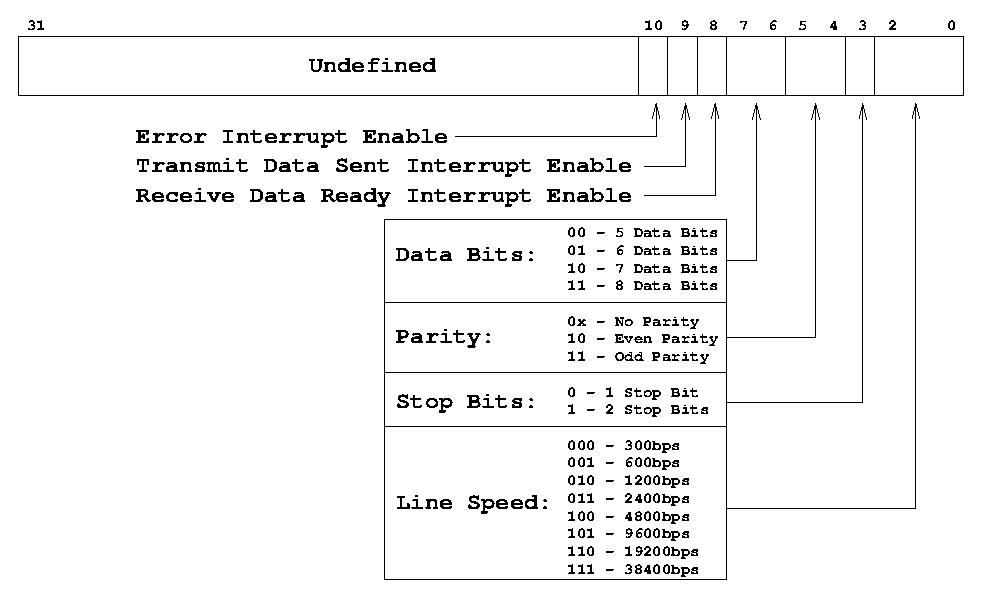
\includegraphics[width=0.8\textwidth]{serial_cr.eps}
\caption{The Serial Control Register}
\label{serial_cr_pic}
\end{center}
\end{figure}

\noindent
eg. To configure a serial interface to operate with no interrupts
enabled, at 9600 bits per second, with 8 data bits, no parity and 1
stop bit, the value `\src{00011000101}' would be written to the
control register.

\newpage
\subsection{Serial Status Register}

The status register is a read-only register, which gives error and
status information about the serial interface. It allows the
programmer to see if data has been received, sent, or if an error
condition is present.

The Transmit Data Sent (TDS) bit will be set to `\src{1}' as soon
as the transmit data register is empty. Checking that this bit is set
allows WRAMP code to ensure that it will not overwrite any data by
placing another character into the transmit data register. This bit
will automatically be cleared if the transmit data register becomes
full.

Similarly, the Receive Data Ready bit will be set to `\src{1}' as soon
as there is new valid data in the receive data register. A read from
the receive data register automatically clears this bit.

\begin{figure}[h]
\begin{center}
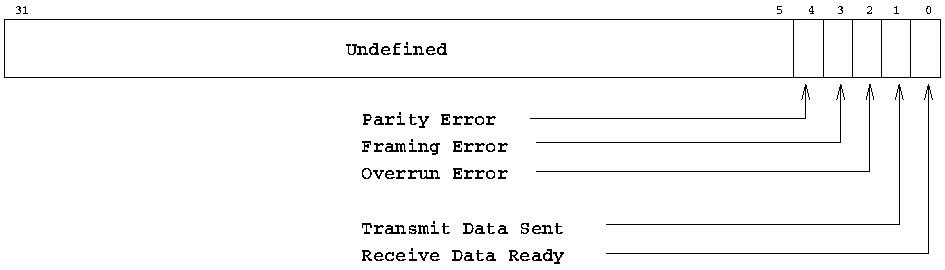
\includegraphics[width=0.8\textwidth]{serial_sr.eps}
\caption{The Serial Status Register}
\label{serial_sr_pic}
\end{center}
\end{figure}

\noindent
eg. If the value `\src{00001}' was read from the status register
then we could determine that a character has been received without
error, and is available in the receive data register.

\subsection{Serial Interrupt Acknowledge Register}

The interrupt acknowledge register is a read/write register. When the
serial interface has generated an interrupt this register allows the
program to determine the reason for the interrupt as well as
acknowledge interrupts that have been dealt with.

To acknowledge an interrupt a zero (`\src{0}') should be written
over the current status field for the type of interrupt being
acknowledged. Most often it will be the desire of the programmer to
acknowledge all of the possible serial port interrupts in one
instruction. This can be achieved by storing register \src{\$0} to
the interrupt acknowledge register.

\begin{figure}[h]
\begin{center}
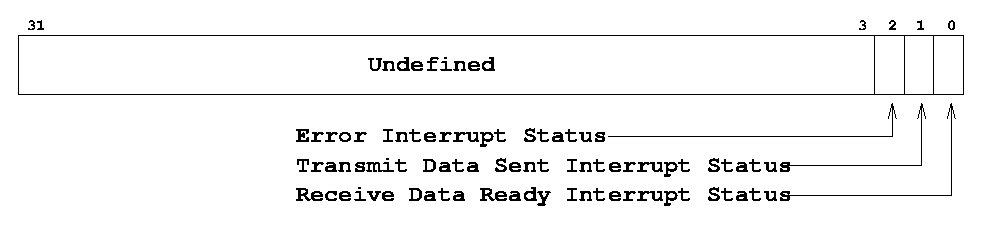
\includegraphics[width=0.8\textwidth]{serial_iack.eps}
\caption{The Serial Interrupt Acknowledge Register}
\label{serial_iack_pic}
\end{center}
\end{figure}

\noindent
eg. If the value `\src{010}' was read from the interrupt
acknowledge register we could determine that the cause of the
interrupt was the transmit data register becoming empty. If the value
`\src{000}' was written to the interrupt acknowledge register all
outstanding serial port interrupts would be acknowledged.

\section{Parallel Interface}

The parallel interface on the REX board provides an input interface
from a bank of 16 on-off switches and three momentary push-buttons, as
well as an output interface to four LED Seven Segment Displays (SSDs),
the 16 LEDs above the switches.
Parallel interrupts, if enabled, will be generated on any switch or
push-button state change.

The programmers view of the parallel interface consists of 10
registers.  The names of these registers and their addresses,
expressed as offsets from the base address, are provided in
Table~\ref{table:parallel_offsets}. The base address for the parallel
port is \src{\LOCPARABASE}. Please note that due to the inclusion of
two more SSDs, the original two SSDs can be addressed from two locations
to allow for both backwards compatibility and having all 4 SSDs in sequential addresses.

\begin{table}[h]
\begin{center}
\begin{tabular}{|l|c|}
\hline
\textbf{Register name} & \textbf{Offset} \\
\hline
Parallel Switch Register & 0 \\
\hline
Parallel Push Button Register & 1 \\
\hline
Parallel Lower Left SSD Register & 2 \\
\hline
Parallel Lower Right SSD Register & 3 \\
\hline
Parallel Control Register & 4 \\
\hline
Parallel Interrupt Acknowledge Register & 5 \\
\hline
Parallel Upper Left SSD Register & 6 \\
\hline
Parallel Upper Right SSD Register & 7 \\
\hline
Parallel Lower Left SSD Register & 8 \\
\hline
Parallel Lower Right SSD Register & 9 \\
\hline
Parallel LED Register & 10 \\
\hline
\end{tabular}
\caption{Parallel Port Register Offsets}
\label{table:parallel_offsets}
\end{center}
\end{table}



\subsection{Parallel Switch Register}

The switch register is a read-only register. A read from this register
returns a bit pattern with bits set corresponding to the switches that
are on.

\begin{figure}[h]
\begin{center}
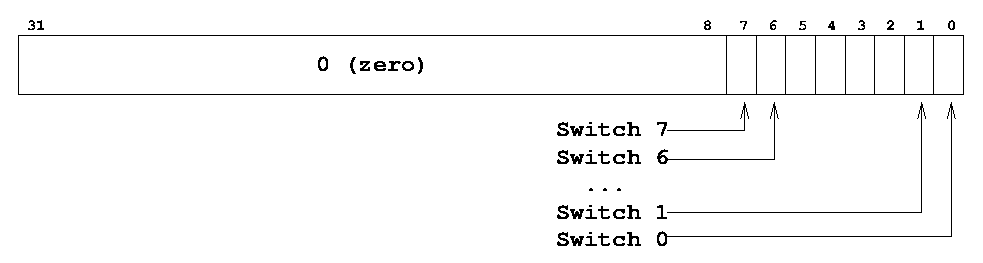
\includegraphics[width=0.8\textwidth]{switch_reg.eps} %%TODO update image to represent 16 switches
\caption{The Switch Register}
\label{switch_reg_pic}
\end{center}
\end{figure}


\subsection{Parallel Push Button Register}

The push button register is a read-only register. A read from this
register returns a bit pattern in the low order 3 bits corresponding
to the push buttons that are currently being depressed.

\begin{figure}[h]
\begin{center}
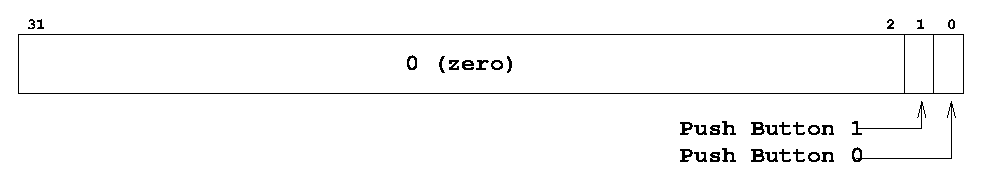
\includegraphics[width=0.8\textwidth]{button_reg.eps} %%TODO update image to represent 3 buttons
\caption{The Push Button Register}
\label{button_reg_pic}
\end{center}
\end{figure}

\subsection{Parallel Left, Right, Upper and Lower SSD Registers}

The four SSD Registers are read/write registers. These
registers contain the value to be displayed on their respective Seven
Segment Display. 

If the hexadecimal to seven-segment decode bit is enabled in the
parallel control register, four bits of input will be decoded into a
single hexadecimal digit and displayed on the seven-segment display.

If the hexadecimal to seven-segment decode bit is turned off, then
each segment can be individually controlled by a single bit of the
input. The displays are made up of seven segments and a decimal point.
The first eight bits of input turn on the segments as shown in
Figure~\ref{fig:ssd}.

\begin{figure}[h]
\begin{center}
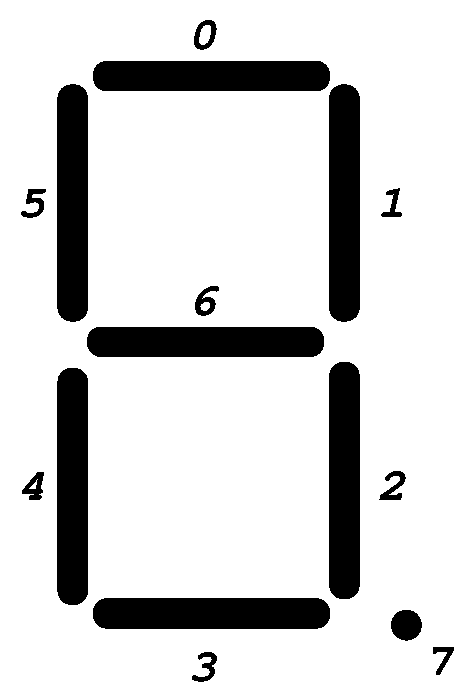
\includegraphics[width=0.12\textwidth]{ssd.eps}
\caption{Seven-segment display bit encoding}
\label{fig:ssd}
\end{center}
\end{figure}

\subsection{Parallel Control Register}

The Parallel Control Register is a read/write register, which allows
for control over the parallel interface.

\begin{figure}[h]
\begin{center}
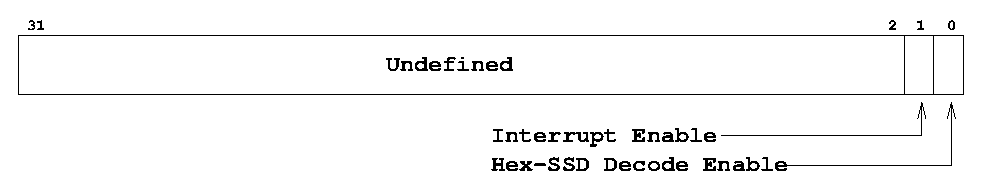
\includegraphics[width=0.8\textwidth]{parallel_cr.eps}
\caption{The Parallel Control Register}
\label{parallel_cr_pic}
\end{center}
\end{figure}

eg. To enable interrupts on switch changes and force hex-SSD decoding
on the displays, a value of `\src{11}' would be written to
the parallel control register.

\subsection{Parallel Interrupt Acknowledge Register}

The Interrupt Acknowledge Register is a read/write register. This
register allows a program to determine the parallel port interrupt
status as well as acknowledge interrupts that have been dealt with.

\begin{figure}[h]
\begin{center}
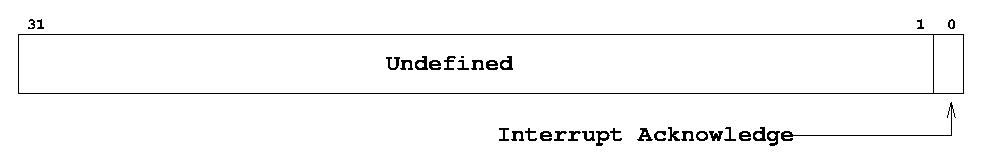
\includegraphics[width=0.8\textwidth]{parallel_iack.eps}
\caption{The Parallel Interrupt Acknowledge Register}
\label{parallel_iack_pic}
\end{center}
\end{figure}

eg. To acknowledge an outstanding parallel port interrupt `\src{0}'
would be written to the parallel interrupt acknowledge register.

\section{Programmable Timer}

The Programmable Timer on the REX board provides for generation of
interrupts at time intervals from about 1ms to 30s, with a resolution
of around 0.5ms.

The timer has an internal 16-bit register. This register is
decremented at a constant rate of 2400Hz.
(Due to the new hardware, a rate of exactly 2400Hz was not attainable.
Instead of picking another whole number we approximated
to maintain backwards compatibility, internally a register counts down from 1302 
at a rate of 6.25MHz, the period of this count yields an approximate 2400.153609831Hz).
Once this register reaches
\src{0x0000} an interrupt is triggered. The starting value for the
timer is controlled by altering the value in the timer load register.

The timer can be configured to automatically reload the starting count
value and continue counting immediately after it expires.

The programmers view of the timer consists of four registers.  The
names of these registers and their addresses, expressed as offsets
from the base address, are provided in
Table~\ref{table:timer_offsets}.  The base address for the timer is
\src{\LOCTIMEBASE}.

\begin{table}[h]
\begin{center}
\begin{tabular}{|l|c|}
\hline
\textbf{Register name} & \textbf{Offset} \\
\hline
Timer Control Register & 0 \\
\hline
Timer Load Register & 1 \\
\hline
Timer Count Register & 2 \\
\hline
Timer Interrupt Acknowledge Register & 3 \\
\hline
\end{tabular}
\caption{Timer Register Offsets}
\label{table:timer_offsets}
\end{center}
\end{table}


\subsection{Timer Control Register}

The Timer Control Register is a read/write register, that allows the
user to enable and control aspects of the timer operation. The timer
has two primary modes of operation, automatic restart and single-shot
mode. If the timer is set to automatic restart, as soon as the timer
expires, an interrupt is triggered and the timer immediately starts
counting down again. In single-shot mode the timer will copy the value
from the timer load register only once when the timer is enabled and
will count down to zero. Once the timer reaches zero an interrupt will
be triggered and the timer will be disabled.

\begin{figure}[h]
\begin{center}
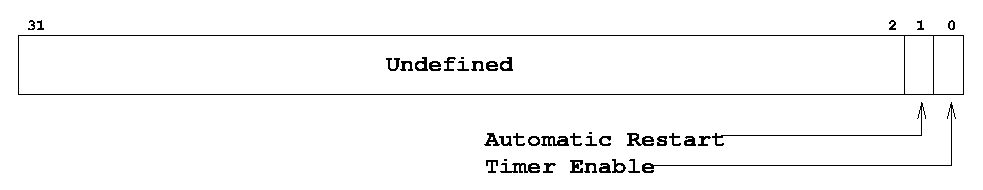
\includegraphics[width=0.8\textwidth]{timer_cr.eps}
\caption{The Timer Control Register}
\label{timer_cr_pic}
\end{center}
\end{figure}

\subsection{Timer Load Register}

The Timer Load Register is a read/write register. This register allows
the user to specify the starting count value. The starting count value
is a 16-bit value with the upper 16 bits being ignored.

\subsection{Timer Count Register}

The Timer Count Register is a read-only register. Reading from this
register returns the current value in the 16-bit internal count
register.

\subsection{Timer Interrupt Acknowledge Register}

The Interrupt Acknowledge Register is a read/write register. This
register allows a program to detect a timer overrun as well as
acknowledge interrupts that have been dealt with.

The overrun detected bit will be set if the timer is set to automatic
restart and the timer expired again before the previous interrupt was
acknowledged. This allows a program to detect if it is unable to
service the timer interrupt fast enough.

The overrun bit must be manually reset by writing a `\src{0}' to
it's location.

\begin{figure}[h]
\begin{center}
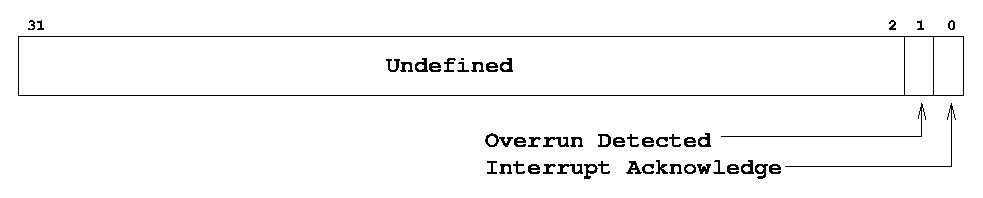
\includegraphics[width=0.8\textwidth]{timer_iack.eps}
\caption{The Timer Interrupt Acknowledge Register}
\label{timer_iack_pic}
\end{center}
\end{figure}

eg. If the value `\src{11}' was read from the interrupt acknowledge
register we could determine that the timer has overrun since we last
acknowledged an interrupt. If `\src{00}' was written to the timer
interrupt acknowledge register we will acknowledge any outstanding
interrupts and ensure the overrun bit is reset to zero.

\subsection{Timer Example}

To configure the timer to interrupt at a specific period the first
step is to calculate the timer load value. This value can be
calculated simply by multiplying the timer frequency by the required
time between interrupts. For example, if we want the timer to generate
an interrupt once every ten seconds we would calculate it as follows:

\begin{center}
Timer Load = 2400Hz * 10s = 24000 = 0x5dc0
\end{center}

Some simple code to initialise the timer to automatically restart and
to interrupt once every ten seconds is given in
Figure~\ref{code:timer_init}.

\begin{figure}[h]
\begin{footnotesize}
\begin{center}
\begin{tabular}{|p{8cm}|}
\hline
\begin{verbatim}
            . . .
           # Make sure there are no old interrupts
           # still hanging around
           sw   $0, 0x72003($0)
           # Put our auto load value in
           addi $11, $0, 0x5dc0
           sw   $11, 0x72001($0)
           # Enable the timer and autorestart
           addi $11, $0, 0x3
           sw   $11, 0x72000($0)
            . . .
\end{verbatim}
\\
\hline
\end{tabular}
\end{center}
\end{footnotesize}
\caption{Simple Timer Initialisation}
\label{code:timer_init}
\end{figure}

